\documentclass[11pt,a4paper]{article}
\usepackage[margin=1.65cm]{geometry}
\usepackage{fontspec}
\setmainfont{TeX Gyre Heros}
\usepackage{amsmath,amssymb,siunitx,booktabs,array,enumitem,multicol}
\usepackage[most]{tcolorbox}
\usepackage{tikz}
\usetikzlibrary{arrows.meta,angles,quotes,decorations.pathmorphing,positioning,calc,patterns}
\usepackage{hyperref,fancyhdr}
\hypersetup{colorlinks=true,linkcolor=black,urlcolor=black,pdftitle={Refraction, Ultrasound, Frequency and Doppler}}
\pagestyle{fancy}\fancyhf{}\lhead{GCSE Physics with Alex}\rhead{18 July 2026}\cfoot{\thepage}
\setlength{\parindent}{0pt}\setlength{\parskip}{5pt}
\setlist{nosep,leftmargin=1.5em}
\newtcolorbox{keybox}[1]{colback=white,colframe=black,boxrule=.7pt,arc=1mm,title=\textbf{#1},fonttitle=\normalsize,breakable}
\newtcolorbox{mistakebox}{colback=black!3,colframe=black,boxrule=.7pt,arc=1mm,title=\textbf{Mistake $\rightarrow$ correction},breakable}
\newcommand{\term}[1]{\textbf{#1}}
\begin{document}
\begin{titlepage}
\centering\vspace*{2.2cm}
{\Huge\bfseries Refraction, Ultrasound, Frequency \& Doppler\par}
\vspace{.5cm}{\Large GCSE Physics lesson-replacement guide\par}
\vspace{1.3cm}
\begin{tcolorbox}[colback=white,colframe=black,width=.82\textwidth]
\centering
\textbf{Student:} Phuc Nguyen\\
\textbf{Tutor:} Alex Kealy\\
\textbf{Lesson date:} 18 July 2026\\
\textbf{Source:} Loom recording (full video analysis) + transcript\\
\textbf{Recording:} ec9e933046484ab49c4f740eff3c6a04
\end{tcolorbox}
\vfill
\textit{A video-first reconstruction of the explanations, board diagrams, student attempts, tutor corrections and exam methods taught in the 62-minute lesson.}
\end{titlepage}
\tableofcontents\newpage

\section{The whole lesson in one page}
This lesson links four ideas through one theme: a wave carries energy, and what we observe depends on how the wave travels. At a material boundary a wave may change speed, change direction or partly reflect. A reflected ultrasound pulse can reveal an unseen boundary. Relative motion changes the spacing of arriving wavefronts, producing the Doppler effect.

\begin{keybox}{Core facts to retrieve}
\begin{itemize}
\item Light travels in straight lines within one uniform medium. At a boundary it may reflect and refract.
\item Reflection obeys $i=r$, with both angles measured from the \term{normal}, not the surface.
\item \term{Refraction} is a change in wave speed on entering a new medium; at an angle, this produces a change in direction.
\item Into a more optically dense medium: slower and \term{towards} the normal. Into a less optically dense medium: faster and \term{away from} the normal.
\item Human hearing is approximately \SIrange{20}{20000}{\hertz}. Ultrasound is above \SI{20000}{\hertz}; infrasound is below \SI{20}{\hertz}.
\item Sound is longitudinal: oscillations are parallel to energy transfer, creating compressions and rarefactions.
\item Echo distance: $d=vt/2$ when $t$ is the complete out-and-back time.
\item Doppler effect: the apparent frequency change caused by relative motion between source and observer. Approaching gives higher observed frequency; receding gives lower observed frequency.
\end{itemize}
\end{keybox}

Alex compared learning to driving a race car around a track: go as fast as possible without sliding off. Forgetting foundational ideas means the ``car'' has crashed and the pace should slow. Use this guide similarly: speed through what you can explain aloud, but stop and reconstruct any diagram or calculation you cannot justify.

\section{Reflection: the launch pad for refraction}
The warm-up recovered vocabulary that refraction questions assume. Phuc correctly said that light travels in straight lines. On Alex's board, a ray approached a flat surface, the dashed normal was perpendicular to it, and a reflected ray left symmetrically.

\begin{center}
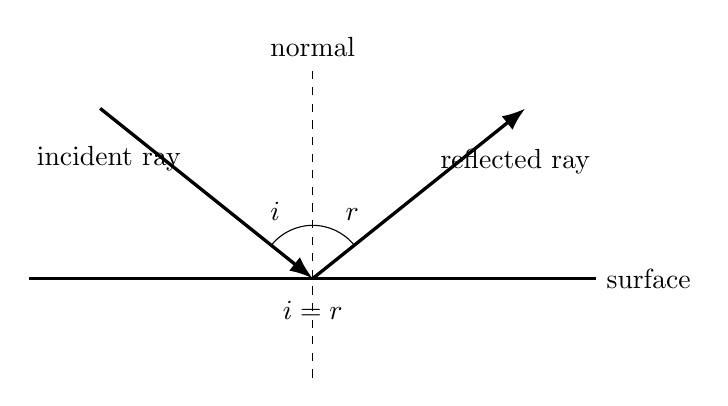
\begin{tikzpicture}[>=Latex,scale=.9]
\draw[thick] (-4,0)--(4,0) node[right]{surface};
\draw[dashed] (0,-1.4)--(0,3) node[above]{normal};
\draw[very thick,->] (-3,2.4)--(0,0) node[pos=.43,above left]{incident ray};
\draw[very thick,->] (0,0)--(3,2.4) node[pos=.55,above right]{reflected ray};
\draw (0,.75) arc (90:141.3:.75) node[midway,above left]{$i$};
\draw (0,.75) arc (90:38.7:.75) node[midway,above right]{$r$};
\node at (0,-.45){$i=r$};
\end{tikzpicture}
\end{center}

Angles must be measured between a ray and the normal. Phuc did not initially recall the completion ``angle of reflection equals ...'', so Alex restored the law $i=r$. Phuc did correctly explain the special shape of a satellite dish: reflected waves are directed to one point. The recalled speed of light in vacuum was \SI{3.00e8}{\metre\per\second}.

\section{Refraction from first principles}
\subsection{What refraction is---and is not}
Alex's lesson definition was precise: refraction is when a wave changes \term{speed} as it changes \term{medium}, causing it to change \term{direction}. The direction change requires the wave to meet the boundary at an angle. If it arrives exactly along the normal, its speed still changes but it continues straight because both sides enter together.

The normal is an imaginary line at $90^\circ$ to the boundary. Always draw it before deciding the bend. From a less optically dense medium into a more optically dense one, the ray slows and bends towards the normal, so the refracted angle is smaller. In the reverse direction it speeds up and bends away, so the refracted angle is larger.

\begin{center}
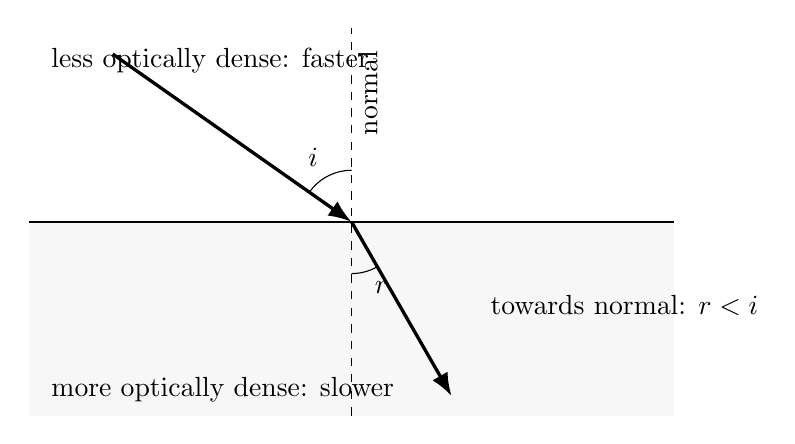
\begin{tikzpicture}[>=Latex,scale=.82]
\fill[black!3] (-5,-3) rectangle (5,0);
\draw[thick] (-5,0)--(5,0);
\draw[dashed] (0,-3)--(0,3);
\node[anchor=west] at (-4.8,2.5){less optically dense: faster};
\node[anchor=west] at (-4.8,-2.6){more optically dense: slower};
\draw[very thick,->] (-3.7,2.6)--(0,0);
\draw[very thick,->] (0,0)--(1.55,-2.7);
\draw (0,.8) arc (90:145:.8) node[midway,above left]{$i$};
\draw (0,-.8) arc (-90:-60:.8) node[midway,below right]{$r$};
\node[right] at (2,-1.3){towards normal: $r<i$};
\node[rotate=90] at (.25,2){normal};
\end{tikzpicture}
\end{center}

\subsection{Why the ray turns: Alex's car analogy}
Imagine the wavefront as the front axle of a car leaving hard tarmac diagonally and entering sand or mud. Wheel 1 reaches the sand first and slows while wheel 2 remains on the fast road. For a short time the wheels move at different speeds, so the car pivots towards the slower side. Light behaves as a wavefront: the part entering the slower medium first lags behind, rotating the front and therefore rotating the direction of travel.

\begin{center}
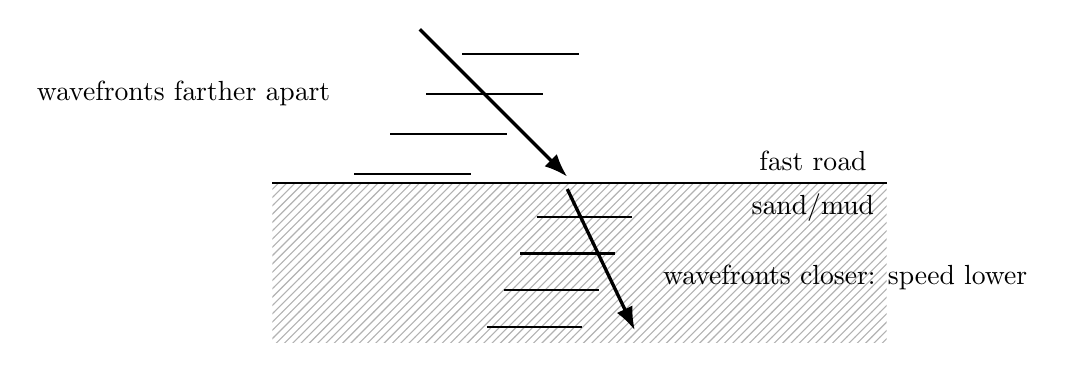
\begin{tikzpicture}[>=Latex,scale=.78]
\fill[pattern=north east lines,pattern color=black!30] (-5,-2.6) rectangle (5,0);
\draw[thick] (-5,0)--(5,0); \node at (3.8,.35){fast road}; \node at (3.8,-.4){sand/mud};
\foreach \y in {2.1,1.45,.8,.15}{\draw[thick] (-3.8+0.9*\y,\y)--(-1.9+0.9*\y,\y);}
\foreach \y in {-.55,-1.15,-1.75,-2.35}{\draw[thick] (-.45+0.45*\y,\y)--(1.1+0.45*\y,\y);}
\draw[very thick,->] (-2.6,2.5)--(-.2,.1); \draw[very thick,->] (-.2,-.1)--(.9,-2.4);
\node[left] at (-3.9,1.45){wavefronts farther apart};
\node[right] at (1.2,-1.55){wavefronts closer: speed lower};
\end{tikzpicture}
\end{center}

Frequency does not change at the boundary: the source still sends the same number of wavefronts each second. Since $v=f\lambda$, a lower speed at unchanged $f$ means a shorter wavelength. The closer wavefronts in the denser medium show this. Alex described refractive index $n$ as a measure of how much a medium bends light, with bonus understanding $n=c/v$. He explicitly said this ratio was not needed for the immediate exam scope.

\subsection{The apparent fish}
In the starter, a boy aimed a spear at where a fish appeared. Phuc first treated it like predicting the fish's movement. Alex corrected the causal story: this is about the \term{path of light}, not the fish swimming. Rays from the fish bend away from the normal as they leave water for air. The eye assumes arriving rays travelled straight, so it traces them backwards to a false, shallower position. Therefore aiming at the apparent fish misses; the real fish is deeper.

\begin{mistakebox}
\textbf{Wrong route:} decide ``towards/away'' from the page direction or from the surface.\\
\textbf{Correction:} identify the medium entered, draw the normal, decide whether speed falls or rises, then compare the new angle with the normal. Do not mix the small reflected portion with the refracted ray, as happened briefly during the car discussion.
\end{mistakebox}

\section{Sound, hearing and ultrasound}
\subsection{Transverse versus longitudinal}
Phuc retrieved the hearing range correctly as \SIrange{20}{20000}{\hertz}, but initially called sound transverse and described perpendicular oscillation. Alex drew both wave types to repair the distinction.

\begin{center}
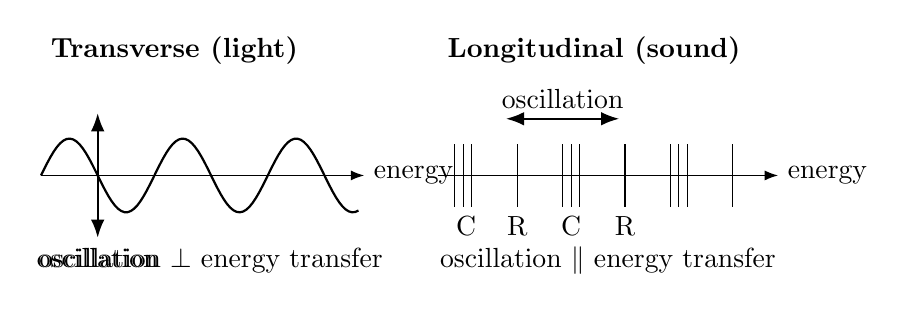
\begin{tikzpicture}[>=Latex,scale=.72]
\node[anchor=west,font=\bfseries] at (-6,2.2){Transverse (light)};
\draw[->] (-6,0)--(-.3,0) node[right]{energy};
\draw[domain=-6:-.4,samples=100,thick] plot (\x,{.65*sin(180*(\x+6))});
\draw[<->,thick] (-5,1.1)--(-5,-1.1) node[below]{oscillation};
\node at (-3,-1.5){oscillation $\perp$ energy transfer};
\node[anchor=west,font=\bfseries] at (1,2.2){Longitudinal (sound)};
\draw[->] (1,0)--(7,0) node[right]{energy};
\foreach \x in {1.3,1.45,1.6,2.4,3.2,3.35,3.5,4.3,5.1,5.25,5.4,6.2}{\draw (\x,-.55)--(\x,.55);}
\draw[<->,thick] (2.2,1)--(4.2,1) node[midway,above]{oscillation};
\node at (1.5,-.9){C};\node at (2.4,-.9){R};\node at (3.35,-.9){C};\node at (4.3,-.9){R};
\node at (4,-1.5){oscillation $\parallel$ energy transfer};
\end{tikzpicture}
\end{center}

A compression is a high-density/high-pressure region; a rarefaction is a low-density/low-pressure region. Frequency is how many complete oscillations pass a point each second, measured in hertz. Phuc also asked whether high-frequency animals ``talk really fast''. Alex corrected this: frequency means pitch/oscillation rate, not speed of speech or wave speed.

Ultrasound is sound above \SI{20000}{\hertz}; infrasound is below \SI{20}{\hertz}. Bats and dolphins emit high-frequency sound and listen for reflections. Alex's intuition was that many wave cycles per second provide detailed timing information, inspiring human imaging and ranging systems.

\subsection{Uses taught}
\begin{itemize}
\item \term{Medical imaging:} pulses enter the body. At boundaries between tissues, part reflects while part continues. Echo times locate boundaries and echo strength helps build an image, for example of a fetus.
\item \term{Industrial testing:} echoes from internal cracks reveal defects without cutting open the object.
\item \term{Echolocation/SONAR:} measure the delay to a seabed or object, using known sound speed.
\item \term{Cleaning jewellery:} high-frequency vibrations in water shake dirt loose. Alex described the water turning brown after a few minutes and stressed that cleaning avoids reactive chemicals on metals or jewels.
\end{itemize}

\section{How pulse--echo imaging and ranging work}
A transducer both sends an ultrasound pulse and detects returning echoes. When a pulse reaches a boundary, only part is reflected; the rest can continue and reflect from deeper boundaries. The display records echo amplitude against time. Earlier echoes correspond to nearer boundaries, not ``faster reflections'': the sound speed in a fixed medium is the same, but the journey is shorter.

\begin{center}
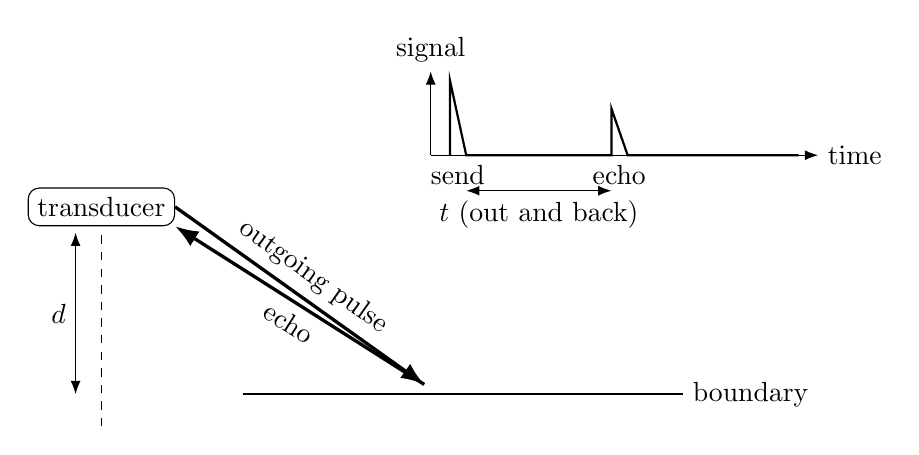
\begin{tikzpicture}[>=Latex,scale=.82]
\node[draw,rounded corners] (T) at (-4,1.4){transducer};
\draw[thick] (-1.8,-1.5)--(5,-1.5) node[right]{boundary};
\draw[very thick,->] (T.east)--(1,-1.35) node[midway,above,sloped]{outgoing pulse};
\draw[very thick,->] (1,-1.35)--(T.south east) node[midway,below,sloped]{echo};
\draw[dashed] (-4,-2)--(-4,1.05);\draw[<->] (-4.4,1)--(-4.4,-1.5) node[midway,left]{$d$};
\begin{scope}[shift={(1.1,2.2)}]
\draw[->] (0,0)--(6,0) node[right]{time};
\draw[->] (0,0)--(0,1.3) node[above]{signal};
\draw[thick] (.3,0)--(.3,1.15)--(.55,0)--(2.8,0)--(2.8,.72)--(3.05,0)--(5.7,0);
\node[below] at (.42,0){send};\node[below] at (2.92,0){echo};
\draw[<->] (.55,-.55)--(2.8,-.55) node[midway,below]{$t$ (out and back)};
\end{scope}
\end{tikzpicture}
\end{center}

The measured time is for two equal legs, each of length $d$:
\[
\text{total distance}=2d=vt\qquad\Longrightarrow\qquad d=\frac{vt}{2}.
\]
Alex repeatedly warned to ask what distance the time represents before substituting. In a sonar drawing the boat sent wavefronts down to the seabed and received them back; the labelled $t$ covered the complete down-and-up path.

\subsection{Turning many echoes into a medical image}
An ultrasound image is not a photograph taken by sound. It is a map constructed from repeated pulse--echo measurements. The transducer sends a short pulse into the body and then listens. At the first tissue boundary, some energy reflects and some transmits. The transmitted part can reach a second boundary, so one emitted pulse can produce several echoes. Electronics measure each delay and use the known speed of sound in tissue to assign a depth. Repeating this along many neighbouring directions builds up a cross-section.

The echo amplitude also matters. A strong echo means a larger fraction was reflected at that boundary; a weak echo means most energy continued. The display can translate these amplitudes into brightness. The important GCSE causal chain is therefore:
\[
\text{boundary}\to\text{partial reflection}\to\text{detected echo}\to\text{time and amplitude}\to\text{position and brightness}.
\]
Alex linked this directly back to reflection and refraction: at a boundary, waves need not do only one thing. Part can reflect while the rest passes through, allowing deeper structures to be found. Coupling gel removes an air gap between transducer and skin, because an unwanted air boundary would strongly interfere with transmission into the body. This final gel detail is standard supporting physics rather than a separate board question; the video-grounded method remains partial reflection plus timed echoes.

High frequency is useful because short wavelengths can resolve small details. The trade-off is that very high-frequency ultrasound is more readily absorbed, so choosing frequency balances detail against penetration depth. For the lesson's exam level, first state that ultrasound is above human hearing, then explain the pulse, reflection at a boundary, detection and timing. Do not claim the baby or crack ``makes'' the ultrasound: the transducer sends it and boundaries return echoes.

\section{The steel-bolt question: attempt, correction, method}
The visible exam question showed a transmitter/detector on a steel bolt and an oscilloscope trace. A transmitted pulse was followed by pulse A after 2.5 divisions and a later pulse B. One division represented \SI{0.000005}{\second}; sound speed in steel was \SI{6000}{\metre\per\second}.

\begin{center}
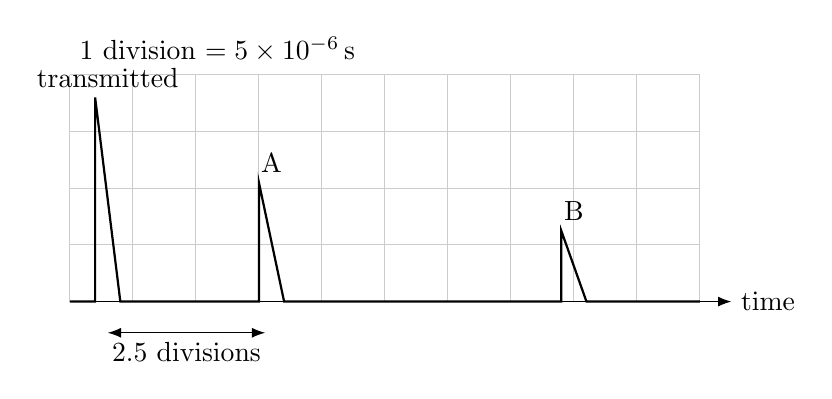
\begin{tikzpicture}[x=.8cm,y=.72cm,>=Latex]
\draw[step=1,black!20] (0,0) grid (10,4);\draw[->] (0,0)--(10.5,0) node[right]{time};
\draw[thick] (0,0)--(.4,0)--(.4,3.6)--(.8,0)--(3,0)--(3,2.1)--(3.4,0)--(7.8,0)--(7.8,1.25)--(8.2,0)--(10,0);
\node[above] at (.6,3.6){transmitted};\node[above] at (3.2,2.1){A};\node[above] at (8,1.25){B};
\draw[<->] (.6,-.55)--(3.1,-.55) node[midway,below]{2.5 divisions};
\node[anchor=west] at (0,4.45){1 division $=\SI{5e-6}{\second}$};
\end{tikzpicture}
\end{center}

\textbf{Part (i): explain A and B.} Phuc initially suggested the crack pulse reflects back ``faster''. Alex redirected attention to two boundaries. Pulse A is produced by reflection from the nearer crack. Some ultrasound continues beyond the crack; pulse B is the later reflection from the far end of the bolt. Return time reveals path length.

\textbf{Part (ii): distance to the crack.} First select A, because the question asks for the crack. Phuc counted five squares towards B; Alex corrected the choice to 2.5 divisions from transmission to A:
\begin{align*}
t&=2.5\times\SI{0.000005}{\second}=1.25\times10^{-5}\,\mathrm{s},\\
vt&=(6000)(1.25\times10^{-5})=\SI{0.075}{\metre}.
\end{align*}
That \SI{0.075}{\metre} is the total head$\to$crack$\to$head path. Phuc had not initially allowed for the return leg. Alex's final correction was therefore
\[
d=\frac{0.075}{2}=\boxed{\SI{0.0375}{\metre}}.
\]
The video-first board evidence gives \SI{0.0375}{\metre}. A transcript-only line later mentions \SI{0.075}{\metre} as the depth; that is the unhalved round-trip value and is superseded by the board calculation.

\begin{mistakebox}
\begin{enumerate}
\item Do not choose B merely because five divisions is easier to count: identify which physical boundary the question names.
\item Do not say A travels faster. In the same steel its speed is fixed; A returns sooner because its path is shorter.
\item Do not stop at $vt$. Label it ``round-trip distance'', then divide by two.
\end{enumerate}
\end{mistakebox}

\section{Doppler effect: from a racing car to redshift}
Alex began with the sound of a Formula 1 car passing: ``nyee-owm''. Phuc recognised that the note falls from high pitch to low pitch. A stationary source emits equally spaced circular wavefronts, so observers in every direction receive the same frequency. A moving source advances between emissions. Ahead, successive fronts are closer together; behind, they are farther apart.

\begin{center}
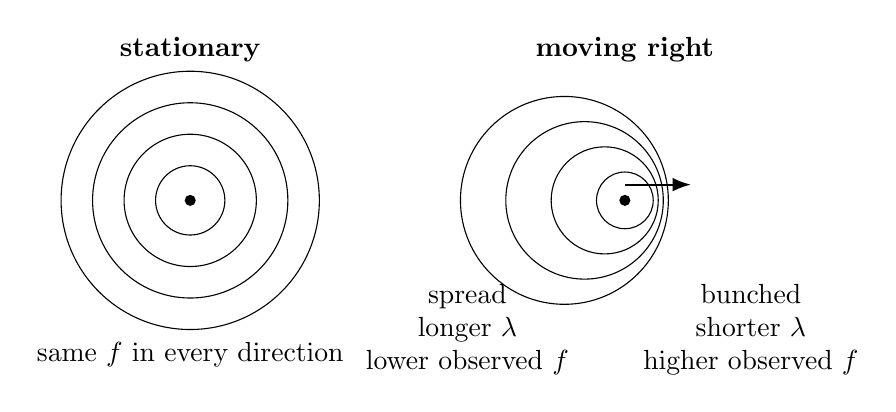
\begin{tikzpicture}[>=Latex,scale=.8]
\node[font=\bfseries] at (-3.7,2.4){stationary};
\fill (-3.7,0) circle (2.5pt);
\foreach \r in {.55,1.05,1.55,2.05}{\draw (-3.7,0) circle (\r);}
\node at (-3.7,-2.45){same $f$ in every direction};
\node[font=\bfseries] at (3.2,2.4){moving right};
\fill (3.2,0) circle (2.5pt);\draw[->,thick] (3.2,.25)--(4.25,.25);
\foreach \i/\r in {0/.45,1/.85,2/1.25,3/1.65}{\draw ({3.2-.32*\i},0) circle (\r);}
\node[align=center] at (5.2,-2.05){bunched\\shorter $\lambda$\\higher observed $f$};
\node[align=center] at (.7,-2.05){spread\\longer $\lambda$\\lower observed $f$};
\end{tikzpicture}
\end{center}

The source does not have to deliberately change its emitted note. Motion changes the rate at which fronts arrive. Phuc then gave the correct explanation: in front of the moving car we hear higher frequency; after it passes and recedes, we hear lower frequency. Alex confirmed this as ``perfect''.

The same principle applies to light. If a star or galaxy moves away, observed wavelengths are stretched towards the red end: \term{redshift}. Alex sketched a nearby source with an example \SI{400}{\nano\metre} wavelength and a distant receding source appearing redder at \SI{500}{\nano\metre}; these were teaching numbers illustrating longer observed wavelength, not a universal conversion.

\begin{center}
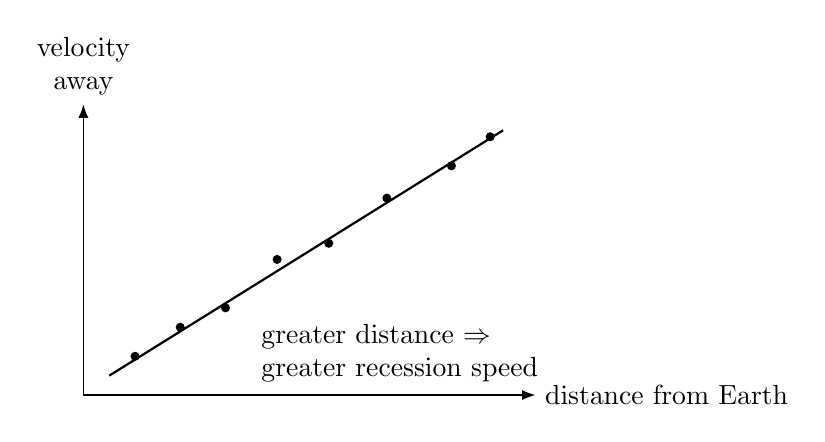
\begin{tikzpicture}[>=Latex,scale=.82]
\draw[->] (0,0)--(7,0) node[right]{distance from Earth};
\draw[->] (0,0)--(0,4.5) node[above,align=center]{velocity\\away};
\foreach \x/\y in {.8/.6,1.5/1.05,2.2/1.35,3/2.1,3.8/2.35,4.7/3.05,5.7/3.55,6.3/4}{\fill (\x,\y) circle (2pt);}
\draw[thick] (.4,.3)--(6.5,4.1);
\node[align=left] at (4.9,.65){greater distance $\Rightarrow$\\greater recession speed};
\end{tikzpicture}
\end{center}

Hubble's positive trend says more distant galaxies recede faster. Alex's rewind analogy supplies the logic: reverse the expansion and the more distant, faster-receding galaxies close the gap; sufficiently far back, matter was concentrated together. This is evidence supporting Big Bang theory. It is not correct to say Hubble's graph alone ``proved'' the Big Bang or that Hubble single-handedly discovered it; Alex corrected this to ``a piece of evidence''.

\section{Exam method and common traps}
\begin{enumerate}
\item \textbf{Draw the normal.} Refraction angles from the surface earn no useful reasoning.
\item \textbf{Name the medium entered.} More optically dense $\to$ slower $\to$ towards; less dense $\to$ faster $\to$ away.
\item \textbf{Separate frequency from speed.} High frequency means more oscillations per second/high pitch, not a faster sound wave in the same medium.
\item \textbf{For echoes, sketch arrows.} If the arrow goes out and back, either halve time first or divide $vt$ by two---never both.
\item \textbf{Interpret traces before calculating.} Earlier pulse means nearer reflector; identify A/B from the named boundary.
\item \textbf{Doppler answers need a causal chain.} Approaching source $\to$ wavefronts closer $\to$ shorter wavelength $\to$ higher observed frequency/pitch.
\item \textbf{Use evidence language.} Redshift and Hubble's trend support expansion and Big Bang theory; they do not amount to absolute proof.
\end{enumerate}

\section{Quick recall and self-test}
\begin{multicols}{2}
\textbf{Questions}
\begin{enumerate}
\item State the law of reflection.
\item Define refraction using three key ideas.
\item Why can normal incidence change speed without bending?
\item What happens entering a denser medium?
\item Explain why a fish appears shallower.
\item State human hearing and ultrasound ranges.
\item Why is sound longitudinal?
\item Name three ultrasound uses.
\item Why does a nearer reflector produce an earlier echo?
\item A pulse at \SI{1500}{\metre\per\second} returns in \SI{0.008}{\second}. Find depth.
\item Explain the high-to-low pitch of a passing car.
\item What does cosmic redshift indicate?
\end{enumerate}
\columnbreak
\textbf{Answers}
\begin{enumerate}
\item $i=r$, measured from the normal.
\item Speed changes on changing medium, causing direction to change at an angle.
\item Both sides of the wavefront change speed simultaneously.
\item It slows and bends towards the normal.
\item Rays bend away leaving water; the eye back-traces them straight to a shallower virtual position.
\item \SIrange{20}{20000}{\hertz}; ultrasound $>\SI{20000}{\hertz}$.
\item Oscillation is parallel to energy transfer.
\item Imaging, flaw detection, sonar/ranging, or cleaning.
\item Same speed, shorter journey.
\item $d=1500(0.008)/2=\SI{6}{\metre}$.
\item Approaching fronts bunch and give higher $f$; receding fronts spread and give lower $f$.
\item The source is receding; widespread redshift supports an expanding universe.
\end{enumerate}
\end{multicols}

\begin{keybox}{Final 30-second memory chain}
Boundary $\to$ speed change $\to$ refraction. Partial reflection $\to$ echo delay $\to$ distance. Source motion $\to$ wavefront spacing change $\to$ apparent frequency change. Receding galaxies $\to$ redshift $\to$ evidence for expansion.
\end{keybox}
\end{document}
